% !TeX program = pdflatex
%
% Generated by scripts/build_latex.py from manuscript.json.
% Prose may be edited here; the tables are regenerated from the analysis, so put
% numeric corrections in the analysis rather than in this file.
%
% Target journal: Journal of Imaging Informatics in Medicine (Springer).
%
\documentclass[11pt,a4paper]{article}

\usepackage[utf8]{inputenc}
\usepackage[T1]{fontenc}
\usepackage{mathptmx}                 % Times text and math; on every TeX install
\usepackage[scaled=0.92]{helvet}
\usepackage[margin=1in]{geometry}
\usepackage{setspace}
\usepackage{graphicx}
\usepackage{booktabs}
\usepackage{longtable}
\usepackage{adjustbox}               % shrinks a table only when it is wider than the text
\usepackage{caption}
\usepackage[hidelinks]{hyperref}
\usepackage{lineno}
\usepackage{xcolor}

\captionsetup{font=small,labelfont=bf,justification=justified,singlelinecheck=false}
\renewcommand{\arraystretch}{1.12}
\setlength{\tabcolsep}{5pt}
\setcounter{secnumdepth}{2}

% Comment out for the camera-ready version.
\linenumbers
\doublespacing

\begin{document}

\begin{center}{\Large\bfseries Data Supplement\par}
{\normalsize Label composition explains whether histology outperforms routine clinicopathological variables: a controlled comparison of four breast cancer risk signatures\par}
{\small Yaqeen Ali, Johannes Gregori\par}
\end{center}
\vspace{1em}
\section{Supplementary Methods}
\subsection{S1. Model and training}
Patch embeddings pass through a shared linear projection and a gated attention module producing one weight per patch; the attention-weighted mean is passed to a regression head predicting the continuous signature score. Training used AdamW at learning rate 1$\times$\$10\textasciicircum{}\{-4\}\$, weight decay 1$\times$\$10\textasciicircum{}\{-4\}\$, gradient-norm clipping at 1.0, batch size one, Huber loss and 20 epochs, with the reported epoch chosen by validation Pearson correlation; the fixed configuration is hidden width 1,024 and dropout 0.25. Patch standardization and target scaling were fitted on training folds only. The four earlier per-target pipelines from which this configuration was taken as the modal setting differed in width, dropout, weight decay, loss and selection rule and used a random patch subsample drawn at every access; the fixed 512-patch pool removes that divergence and the per-access randomness.

\subsection{S2. Partition}
Multi-label stratification places patients one at a time, rarest label first, into whichever fold is furthest below its target count for that label, so every fold carries a similar positive rate for all four binary targets and for ER status simultaneously [22]; with four targets plus ER, an ordinary stratified split produces folds in which one target has a single-class test set. The inner three-fold split for epoch selection was drawn by the same procedure inside each training set.

\subsection{S3. Comparator sensitivity and incremental analyses}
The tuned comparator chose the L2 penalty from C $\in$ \{0.01, 0.03, 0.1, 0.3, 1\} by inner three-fold cross-validation within each training fold. The stacked model entered the out-of-fold histology score, standardized, as a seventh variable into the same tuned logistic model, refitted inside each fold, and was compared with the tuned clinical model by paired bootstrap on the same folds. Because that model must be estimated from few minority-class cases, the association was also tested on all 81 patients by a likelihood-ratio test for the histology score added to the six variables, reported as an odds ratio per standard deviation. Events per variable are the minority-class count divided by seven. The tuned penalty changed the Oncotype comparator from 0.464 to 0.495 and the ROR-S comparator from 0.710 to 0.746, and left ROR-P and MammaPrint essentially unchanged. For Oncotype the unadjusted association was present (odds ratio 1.93 per SD, 1.03 to 3.60; p = 0.033) but the adjusted one uninformative in either direction.

\subsection{S4. Minimum detectable difference}
The minimum detectable difference between two AUCs measured on the same patients was computed from the Hanley--McNeil standard error [28, 29] assuming both AUCs near 0.80, a correlation of 0.5 between them, two-sided $\alpha$ = 0.05 and 80\% power, at the observed class balance of each target: 0.135 to 0.154 in the full cohort, 0.165 to 0.221 in the ER-positive, HER2-negative subgroup, and about 0.04 to 0.05 at n $\approx$ 900 with the same class balance.

\subsection{S5. Repeated cross-validation}
The entire locked pipeline --- the same fixed configuration, model, fixed patch pools and fold-honest C = 1 clinicopathological comparator --- was rerun under five independently drawn multi-label stratified five-fold partitions, changing only the seed that draws the outer partition and the inner epoch-selection split. The first seed is the locked seed, so repeat 0 reproduces the primary numbers exactly and serves as a check on the harness. This measures how much the point estimates move with the split; it adds no patients, so the confidence intervals and multiplicity adjustment of the primary analysis are unchanged.

\section{Supplementary Results}
\subsection{S6. Calibration and stability}
Calibration slopes for the continuous predictions were 0.658 (Oncotype), 0.815 (ROR-P), 0.983 (ROR-S) and 1.124 (MammaPrint) (Table S1). A slope below one means the predictions are spread more widely than the observed scores warrant --- the over-dispersion expected of a model fitted to a small sample --- so the Oncotype predictions are the least well calibrated and the MammaPrint predictions mildly compressed. Per-fold variability was modest for MammaPrint (AUC 0.955 $\pm$ 0.037) and larger for Oncotype (0.749 $\pm$ 0.105); per-fold SDs of 0.037 to 0.105 show that a single five-fold draw is a coarse instrument at this sample size. The MammaPrint per-fold mean sits above its pooled value because the predicted scale shifts between folds, a within-fold ranking that pooling penalizes.

\subsection{S7. Performance within ER-positive disease}
Restriction to ER-positive, HER2-negative disease (n = 56) --- the population in which Oncotype DX and the PAM50 scores are principally used, and most of the MammaPrint indication --- applies to the evaluation set only; the models were developed on the full cohort, so these figures are not what a model developed within the indication would achieve (Table S2). This is the group in which the six variables carry least information, since two of them are constant within it, and it is where the morphological signal does the most work. Within ER-positive disease as a whole the MammaPrint AUC rests on four negatives.

\subsection{S8. Pre-extracted radiomic feature arm}
Nested cross-validation gave AUC 0.593 for Oncotype (95\% CI, 0.429 to 0.752), 0.628 for MammaPrint (0.454 to 0.790), 0.588 for ROR-P (0.454 to 0.721) and 0.637 for ROR-S (0.510 to 0.760); the non-nested procedure returned 0.656, 0.749, 0.610 and 0.692 on the same data, an optimism of +0.022 to +0.121 AUC (Table S3). Three of the four nested intervals include chance; the ROR-S interval sits just above it. The optimism was largest for MammaPrint. On this cohort the arm has at most a marginal signal, and most of the signal the conventional procedure reports is an artifact of selecting and scoring on the same data. The arm is a methodological control: its role is to show that the selection-bias magnitude described in the literature is directly observable on the same patients and folds as the histology analysis.

\subsection{S9. Effect of the design choices}
Under the earlier per-target pipelines, with per-target partitions, per-target tuned hyperparameters and a random patch subsample at every access, the same comparator gave margins of +0.155 for Oncotype ($-$0.005 to 0.314; p = 0.057), +0.173 for ROR-P, +0.066 for ROR-S ($-$0.075 to 0.205; p = 0.349) and +0.014 for MammaPrint ($-$0.055 to 0.082; p = 0.673): Oncotype was a marginal result, ROR-S was null and MammaPrint showed a small positive margin. Under one shared partition, one configuration and a fixed patch pool, Oncotype became the strongest result, ROR-S gained a nominally significant margin, ROR-P was unchanged and MammaPrint's margin became negative (Table S4). Separately, nesting the radiomic feature selection removed most of that arm's apparent performance.

\subsection{S10. Repeated cross-validation}
Across the five partitions the histology AUC and the margin over the clinicopathological model are given as mean $\pm$ SD with the range (Table S5). The Oncotype, ROR-P and ROR-S margins were positive in all five draws; the MammaPrint margin straddled zero, positive in two of five.

\clearpage
\section*{Supplementary tables}
\begin{spacing}{1.0}
\begin{table}[htbp]\centering\small
\caption*{\textbf{Table S1.} Agreement with the continuous score, per-fold stability and calibration (n = 82). Calibration is the regression of observed on predicted values: a slope below one means the predictions are spread more widely than the observed scores, a slope above one that they are compressed toward the mean.}
\begin{adjustbox}{max width=\textwidth}
\begin{tabular}{@{}lcccc@{}}
\toprule
\textbf{Signature} & \textbf{Pearson r (95\% CI)} & \textbf{AUC per fold (mean $\pm$ SD)} & \textbf{Calibration slope} & \textbf{Intercept} \\
\midrule
Oncotype & 0.449 (0.295--0.591) & 0.749 $\pm$ 0.105 & 0.658 & 21.30 \\
ROR-P & 0.589 (0.426--0.728) & 0.844 $\pm$ 0.087 & 0.815 & 5.04 \\
ROR-S & 0.695 (0.566--0.796) & 0.843 $\pm$ 0.094 & 0.983 & 0.71 \\
MammaPrint & 0.766 (0.644--0.848) & 0.955 $\pm$ 0.037 & 1.124 & 0.00 \\
\bottomrule
\end{tabular}
\end{adjustbox}\end{table}

\begin{table}[htbp]\centering\footnotesize
\caption*{\textbf{Table S2.} Performance restricted to ER-positive and ER-positive, HER2-negative disease. Restriction applies to the evaluation set only; models were developed on the full cohort. n (positives) per subgroup. Clinical AUCs are given for the pre-declared and the tuned comparator. ``Not evaluable'': all 56 patients share one MammaPrint label, so no AUC is defined; the ER-positive MammaPrint row rests on four negatives.}
\begin{adjustbox}{max width=\textwidth}
\begin{tabular}{@{}lccccc@{}}
\toprule
\textbf{Signature} & \textbf{Cohort} & \textbf{n (pos.)} & \textbf{Histology AUC} & \textbf{Clinical AUC, pre-declared} & \textbf{Clinical AUC, tuned} \\
\midrule
Oncotype & All & 81 (67) & 0.744 & 0.464 & 0.495 \\
 & ER-positive & 70 (56) & 0.708 & 0.367 & 0.403 \\
 & ER-positive, HER2-negative & 56 (43) & 0.673 & 0.279 & 0.297 \\
ROR-P & All & 81 (50) & 0.815 & 0.655 & 0.642 \\
 & ER-positive & 70 (39) & 0.770 & 0.558 & 0.541 \\
 & ER-positive, HER2-negative & 56 (30) & 0.756 & 0.554 & 0.533 \\
ROR-S & All & 81 (32) & 0.834 & 0.710 & 0.746 \\
 & ER-positive & 70 (21) & 0.763 & 0.558 & 0.612 \\
 & ER-positive, HER2-negative & 56 (13) & 0.673 & 0.360 & 0.496 \\
MammaPrint & All & 81 (67) & 0.892 & 0.934 & 0.934 \\
 & ER-positive & 70 (66) & 0.799 & 0.818 & 0.818 \\
 & ER-positive, HER2-negative & 56 (56) & not evaluable & not evaluable & not evaluable \\
\bottomrule
\end{tabular}
\end{adjustbox}\end{table}

\begin{table}[htbp]\centering\small
\caption*{\textbf{Table S3.} Pre-extracted radiomic feature arm: nested versus conventional non-nested cross-validation, on the same patients and the same folds as the histology arm (n = 82). Three of the four nested intervals include chance; the ROR-S interval sits just above it. No clinicopathological comparator is reported for this arm because the nested AUCs are at or near chance, so a head-to-head comparison would be uninformative.}
\begin{adjustbox}{max width=\textwidth}
\begin{tabular}{@{}lccc@{}}
\toprule
\textbf{Target} & \textbf{Nested AUC (95\% CI)} & \textbf{Non-nested AUC} & \textbf{Optimism} \\
\midrule
Oncotype & 0.593 (0.429--0.752) & 0.656 & +0.063 \\
MammaPrint & 0.628 (0.454--0.790) & 0.749 & +0.121 \\
ROR-P & 0.588 (0.454--0.721) & 0.610 & +0.022 \\
ROR-S & 0.637 (0.510--0.760) & 0.692 & +0.054 \\
\bottomrule
\end{tabular}
\end{adjustbox}\end{table}

\begin{table}[htbp]\centering\small
\caption*{\textbf{Table S4.} Effect of the design choices: the earlier per-target pipelines against the locked design. Provisional: each target on its own cross-validation partition with its own tuned hyperparameters and a random patch subsample drawn at every access (n = 82, neoadjuvant case still included). Locked: one shared partition, one configuration, a fixed patch pool (n = 81). The comparator, HER2 rule, bootstrap and seed are identical in both columns; only the imaging-side design differs. Gain is over the pre-declared clinicopathological model.}
\begin{adjustbox}{max width=\textwidth}
\begin{tabular}{@{}lcccc@{}}
\toprule
\textbf{Signature} & \textbf{Provisional AUC} & \textbf{Provisional gain (95\% CI); p} & \textbf{Locked AUC} & \textbf{Locked gain (95\% CI); p} \\
\midrule
Oncotype & 0.703 & +0.155 ($-$0.005 to 0.314); 0.057 & 0.744 & +0.280 (0.133 to 0.435); <0.001 \\
ROR-P & 0.807 & +0.173 (0.023 to 0.328); 0.027 & 0.815 & +0.160 (0.012 to 0.300); 0.036 \\
ROR-S & 0.779 & +0.066 ($-$0.075 to 0.205); 0.349 & 0.834 & +0.124 (0.013 to 0.246); 0.028 \\
MammaPrint & 0.955 & +0.014 ($-$0.055 to 0.082); 0.673 & 0.892 & $-$0.042 ($-$0.134 to 0.034); 0.313 \\
\bottomrule
\end{tabular}
\end{adjustbox}\end{table}

\begin{table}[htbp]\centering\small
\caption*{\textbf{Table S5.} Repeated cross-validation. The entire locked pipeline --- same fixed configuration, same model, same fixed patch pools, same fold-honest C = 1 clinicopathological comparator --- was rerun under five independently drawn multi-label stratified five-fold partitions (n = 81); the first is the locked partition and reproduces the primary numbers exactly. Values are the mean $\pm$ SD across the five partitions with the range in brackets. This measures how much the point estimate moves with the split, not statistical significance, and does not add patients: the confidence intervals and multiplicity adjustment of Table 2 are unchanged.}
\begin{adjustbox}{max width=\textwidth}
\begin{tabular}{@{}lccc@{}}
\toprule
\textbf{Signature} & \textbf{Histology AUC, mean $\pm$ SD (range)} & \textbf{Gain over clinical, mean $\pm$ SD (range)} & \textbf{Draws with gain > 0} \\
\midrule
Oncotype & 0.718 $\pm$ 0.067 (0.633--0.814) & +0.213 $\pm$ 0.051 (+0.162 to +0.280) & 5 / 5 \\
ROR-P & 0.793 $\pm$ 0.016 (0.772--0.815) & +0.199 $\pm$ 0.045 (+0.145 to +0.249) & 5 / 5 \\
ROR-S & 0.791 $\pm$ 0.034 (0.744--0.834) & +0.111 $\pm$ 0.046 (+0.050 to +0.167) & 5 / 5 \\
MammaPrint & 0.903 $\pm$ 0.025 (0.877--0.941) & $-$0.006 $\pm$ 0.048 ($-$0.061 to +0.063) & 2 / 5 \\
\bottomrule
\end{tabular}
\end{adjustbox}\end{table}

\end{spacing}
\clearpage
\section*{Supplementary figures}
\begin{figure}[htbp]\centering
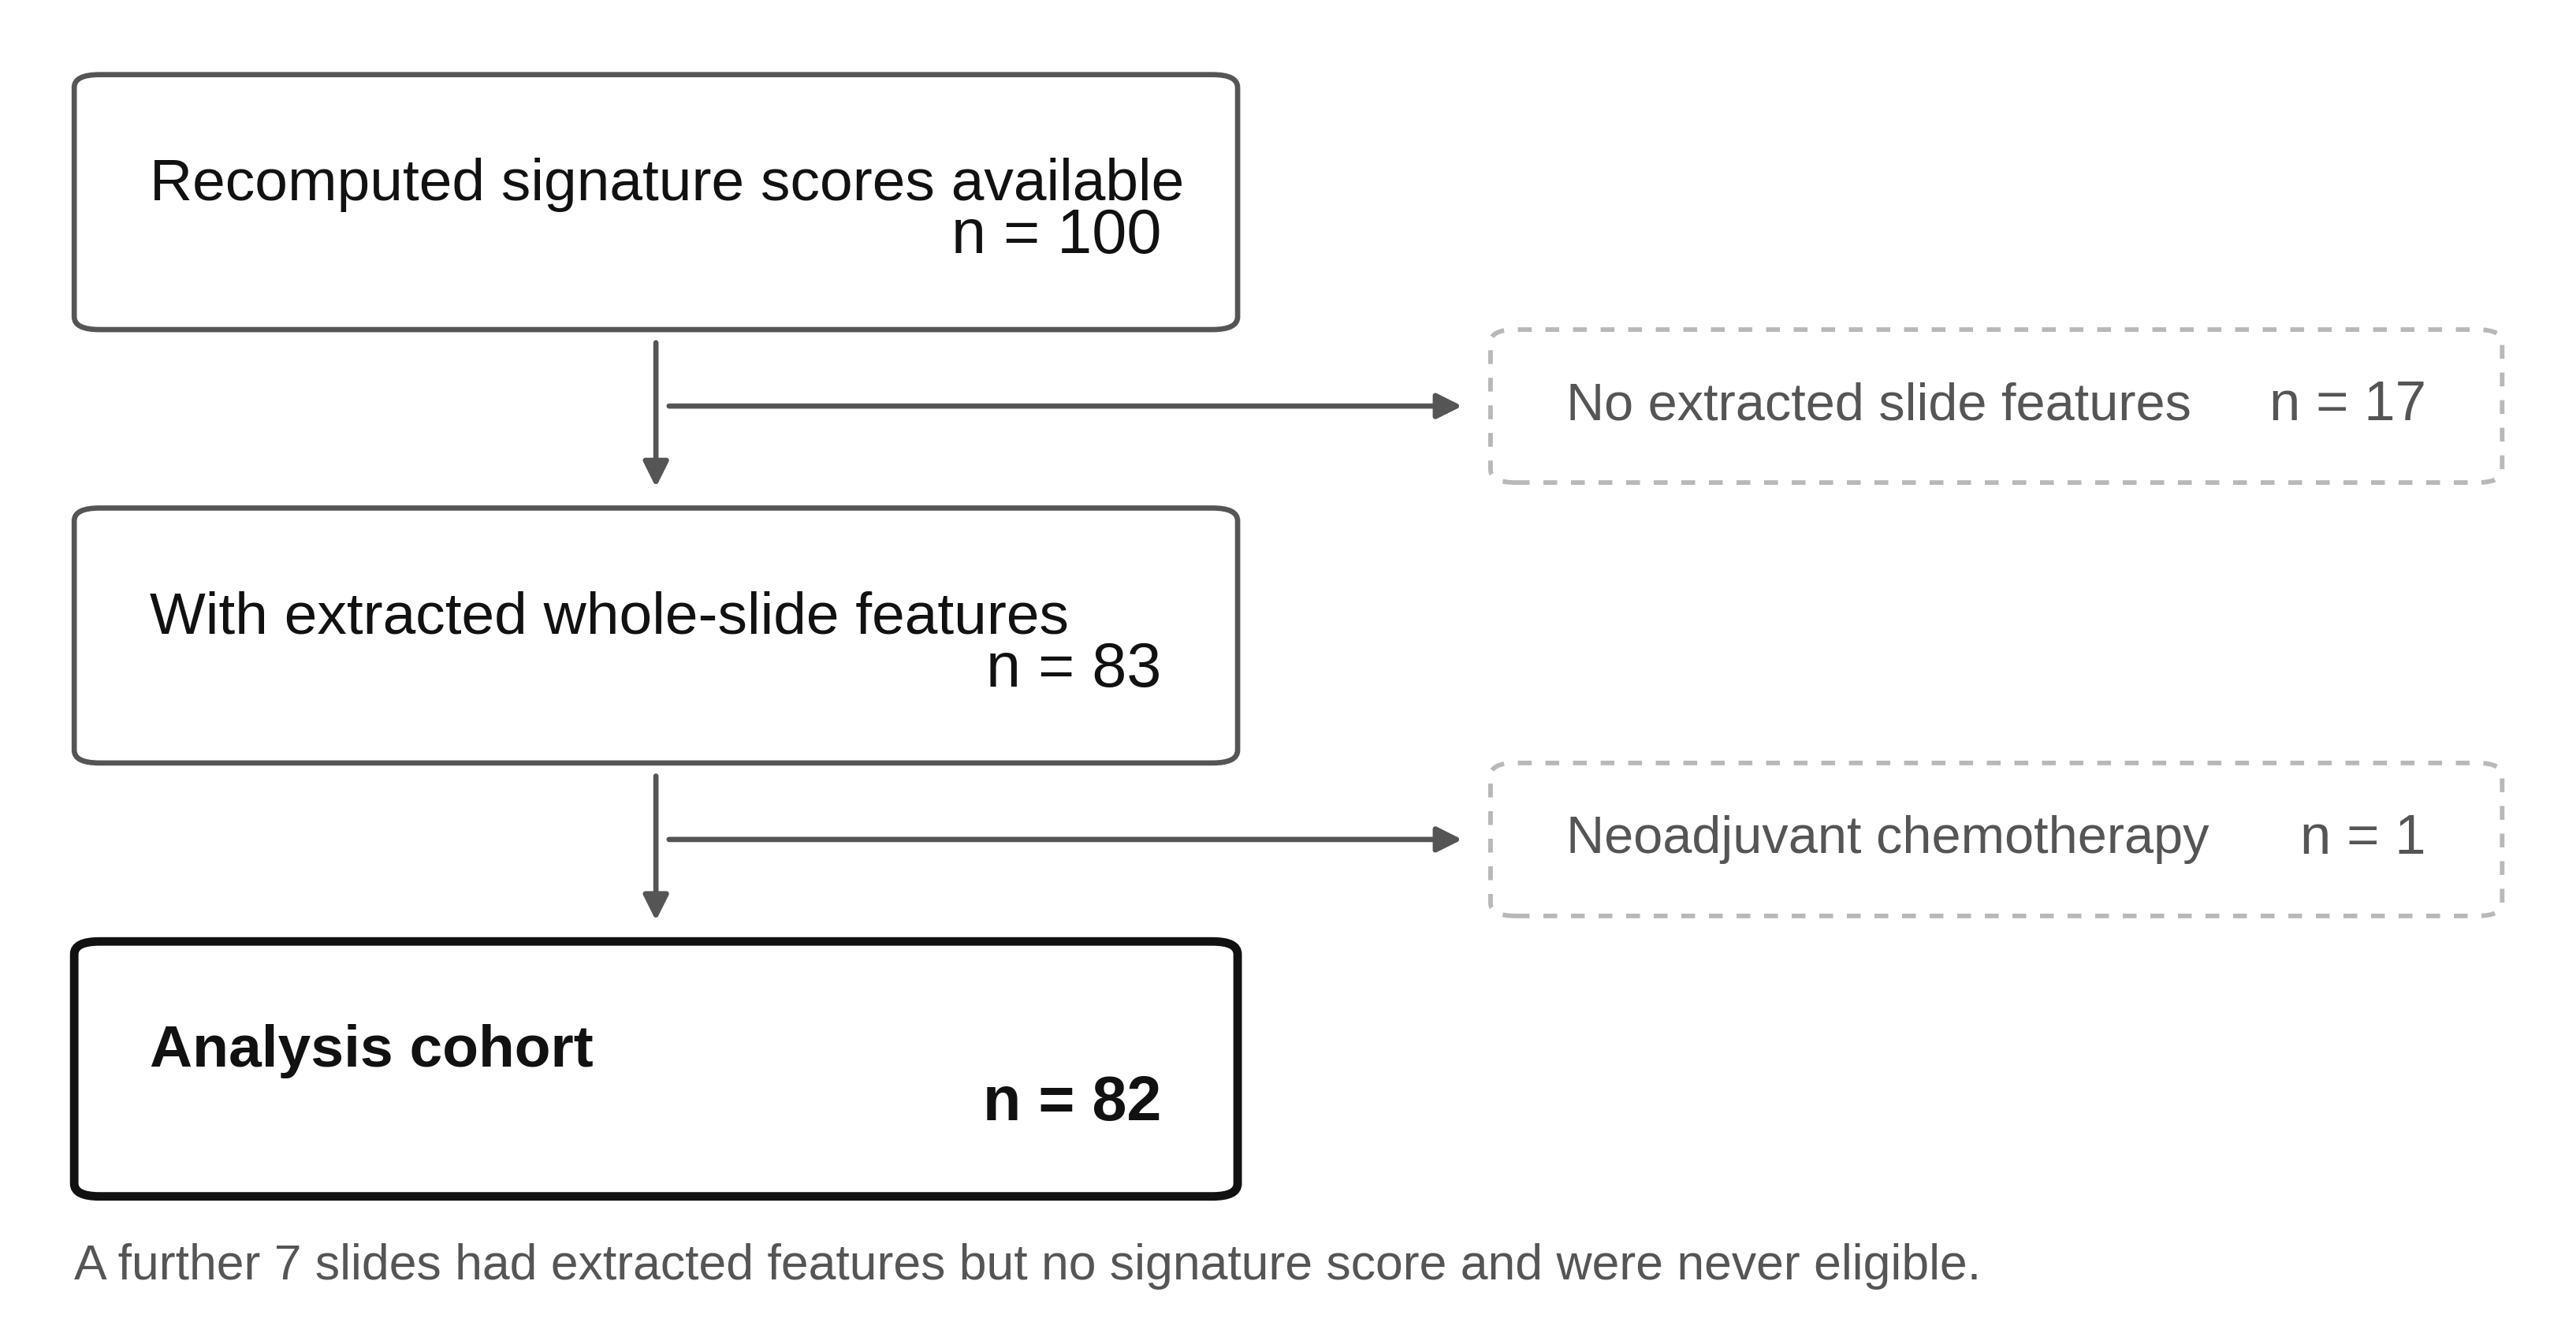
\includegraphics[width=0.95\textwidth]{figures/FigS1.png}
\caption*{\textbf{Fig S1.} Cohort flow. The analysis cohort is the intersection of two lists: patients with recomputed signature scores and patients with extracted whole-slide features. Neither can be enlarged from the available data.}
\end{figure}
\clearpage
\end{document}
